\documentclass[12pt]{article}
% This first part of the file is called the PREAMBLE. It includes
% customizations and command definitions. The preamble is everything
% between \documentclass and \begin{document}.

\usepackage[margin=1in]{geometry}  % set the margins to 1in on all sides
\usepackage{graphicx}              % to include figures
\usepackage{amsmath}               % great math stuff
\usepackage{amsfonts}              % for blackboard bold, etc
\usepackage{amsthm}                % better theorem environments

\usepackage{rotating} % for sideway table
\usepackage{xcolor}
\usepackage{hyperref}
\hypersetup{
    colorlinks,
    linkcolor={red!50!black},
    citecolor={blue!50!black},
    urlcolor={blue!80!black}
}
\usepackage{cleveref}

\usepackage{array,tabularx}

\newenvironment{conditions*}
  {\par\vspace{\abovedisplayskip}\noindent
   \tabularx{\columnwidth}{>{$}l<{$} @{${}={}$} >{\raggedright\arraybackslash}X}}
  {\endtabularx\par\vspace{\belowdisplayskip}}
  
\usepackage{float}
\restylefloat{table}

% various theorems, numbered by section

\newtheorem{thm}{Theorem}[section]
\newtheorem{lem}[thm]{Lemma}
\newtheorem{prop}[thm]{Proposition}
\newtheorem{cor}[thm]{Corollary}
\newtheorem{conj}[thm]{Conjecture}

\DeclareMathOperator{\id}{id}

\newcommand{\bd}[1]{\mathbf{#1}}  % for bolding symbols
\newcommand{\RR}{\mathbb{R}}      % for Real numbers
\newcommand{\ZZ}{\mathbb{Z}}      % for Integers
\newcommand{\col}[1]{\left[\begin{matrix} #1 \end{matrix} \right]}
\newcommand{\comb}[2]{\binom{#1^2 + #2^2}{#1+#2}}

% bibliography
\usepackage{natbib}
\bibpunct{(}{)}{;}{a}{}{,} % no comma between author and year

\title{Conflict Prediction with Spike and Slab prior}
\author{Anh Le}

\begin{document}
\maketitle

\begin{figure}
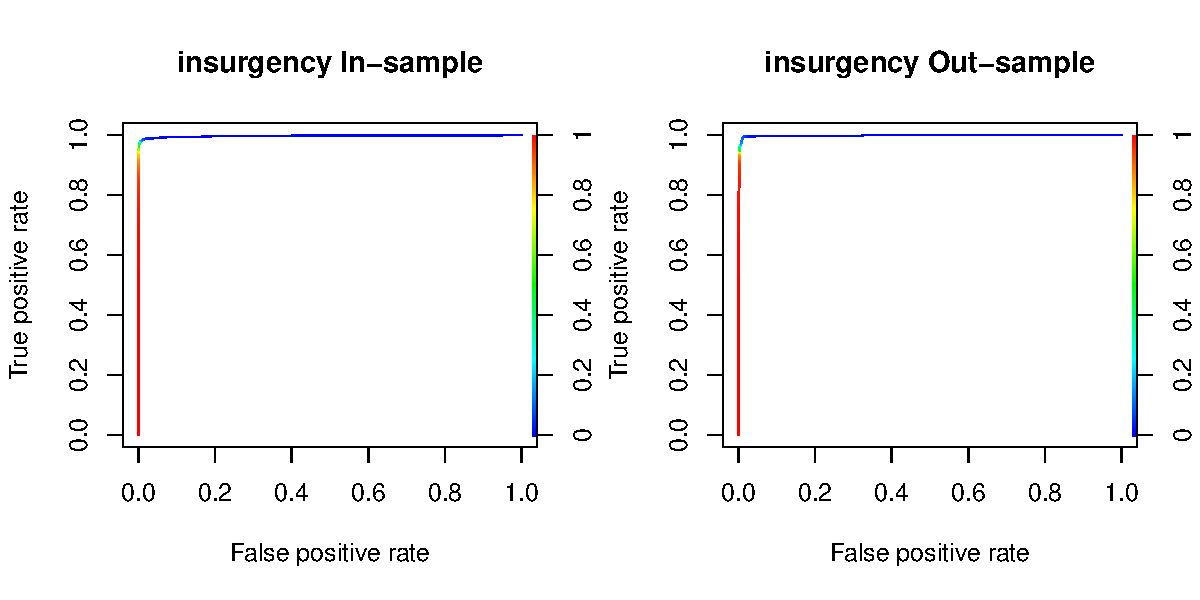
\includegraphics[width=\textwidth]{fig/roc_insurgency}
\end{figure}

\begin{figure}
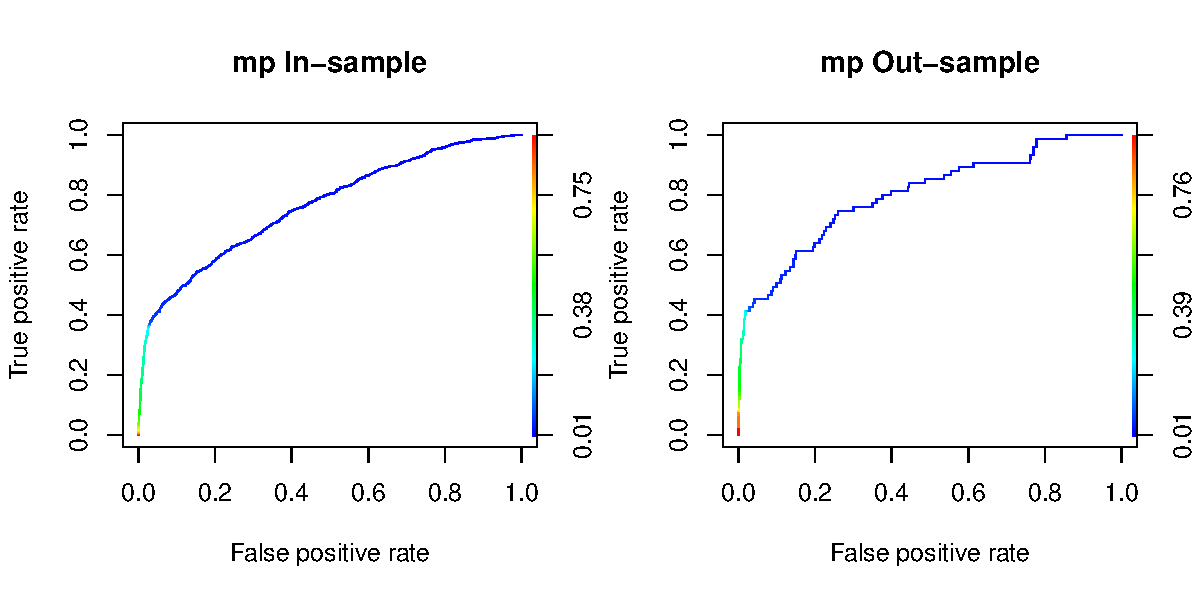
\includegraphics[width=\textwidth]{fig/roc_mp}
\end{figure}

\begin{table}
\centering
% latex table generated in R 3.1.2 by xtable 1.7-4 package
% Fri Dec  5 14:50:23 2014
\begin{tabular}{rrrrrr}
  \hline
 & insurgency & rebellion & dpc & erv & mp \\ 
  \hline
brier & 0.005 & 0.006 & 0.042 & 0.008 & 0.036 \\ 
  auc.C & 0.996 & 0.999 & 0.927 & 0.989 & 0.764 \\ 
  precision & 0.981 & 0.957 & 0.789 & 0.961 & 0.548 \\ 
  recall & 0.767 & 0.769 & 0.410 & 0.681 & 0.068 \\ 
   \hline
\end{tabular}

\caption{In-sample predictive performance}
\end{table}

\begin{table}
\centering
% latex table generated in R 3.1.2 by xtable 1.7-4 package
% Mon Dec  1 05:33:13 2014
\begin{tabular}{rrrrr}
  \hline
 & insurgency & rebellion & dpc & erv \\ 
  \hline
brier & 0.009 & 0.019 & 0.088 & 0.034 \\ 
  auc.C & 0.997 & 0.903 & 0.860 & 0.977 \\ 
  precision & 0.976 & 0.906 & 0.642 & 0.905 \\ 
  recall & 0.946 & 0.784 & 0.460 & 0.480 \\ 
   \hline
\end{tabular}

\caption{Out-sample predictive performance}
\end{table}

\end{document}
